\documentclass[11pt,a4paper]{article}

\usepackage[utf8]{inputenc}
\usepackage[T1]{fontenc}
\usepackage{lmodern}
\usepackage{amsmath}
\usepackage[margin=2.3cm]{geometry}
\usepackage{microtype}
\usepackage{booktabs}
\usepackage{tabularx}
\usepackage{array}
\newcolumntype{Y}{>{\raggedright\arraybackslash}X}
\usepackage{multirow}
\usepackage{graphicx}
\usepackage{xcolor}
\usepackage{tikz}
\usetikzlibrary{positioning,fit,arrows.meta,shapes.geometric,backgrounds,calc}
\usepackage{forest}
\usepackage{pgfplots}
\pgfplotsset{compat=1.16}
\usepackage[numbers,sort&compress]{natbib}
\usepackage{caption}
\usepackage{enumitem}
\setlist{itemsep=1pt,topsep=3pt}
\usepackage[hidelinks]{hyperref}
\usepackage{xurl}
\usepackage[htt]{hyphenat}   % allow line breaks inside \texttt
\emergencystretch=3em

% Visible marker for content the repository does not provide
\newcommand{\TODO}[1]{\textcolor{red}{\textbf{TODO(#1)}}}
\newcommand{\code}[1]{\texttt{#1}}
\newcommand{\rid}[1]{\textsf{#1}}                 % Wazuh rule id
\newcommand{\metric}[1]{\texttt{\small #1}}

\title{Threat Detection, Monitoring and Prevention\\in a Location-Aware Service Platform\\[4pt]
  \large Security in Large Scale Systems --- Project 1}
\author{\TODO{group member names and student numbers}\\
  Universidade de Aveiro, DETI}
\date{November 2026}

\begin{document}
\maketitle

\begin{abstract}
We designed, deployed and attacked a small service-based IoT platform (temperature sensors,
ingestion, storage, analytics and a service registry) that is built to grow across locations. Every
element gets a hierarchical name, from \emph{service instance} up to \emph{country}, that is the
same in the registry, in Prometheus, in Wazuh and in every log line, so any metric or security event
points to where it came from. The platform runs as Docker images in a two-node Kubernetes (k3s)
cluster in which each node is a data centre; an earlier one-container-per-service deployment on
Incus serves as a baseline. Prometheus monitors every instance, correlates symptoms into a single
root-cause alert, and exports per-location aggregates that cut federation traffic to under 1\% of a
raw federation. Wazuh detects three syllabus threats (a massive HTTP denial of service, junk email,
and DNS hijacking) and responds automatically: a tampered DNS zone was restored in
0.28~s on average over five runs, and flood sources were blocked within about 3~s in three of five
runs, but not when the attacked service was too overloaded to log the attack. We report what worked,
what failed (including defences that caused their own outage), and where the design stops scaling.
\end{abstract}

\tableofcontents
\newpage

\section{Introduction}
\label{sec:intro}

Large-scale service platforms, such as telecom and cloud operators or IoT back-ends, have two
problems the small version of the same system does not have. First, \emph{finding things}: with
hundreds of instances spread over sites, an alert is useless unless it says which instance, on
which machine, in which data centre. Second, \emph{defending at scale}: the defences must work on
every instance at once, must not overload the links between sites with monitoring traffic, and must
not hurt the system they protect.

The objective of this project is to design and run a service-based architecture that scales to
large scale, monitor it with Prometheus, and integrate it with a SIEM (Wazuh) that detects three
types of incident from the course syllabus and responds automatically. The system is a small IoT
pipeline in which temperature sensors send readings to an ingestion service, which stores them
through a storage service, while an analytics service computes statistics and a registry provides
naming and discovery. The platform runs as Docker images in a two-node Kubernetes (k3s) cluster in
which each node is a different data centre. An earlier deployment with one Incus container per
service was kept as a baseline, and every test runs unchanged on both.

\paragraph{Contributions.}
\begin{itemize}
  \item A hierarchical naming scheme (\emph{instance.node.rack.dc.region.country}) that is used
        unchanged by the registry, the metrics, the SIEM agents and the logs, so the source of any
        event can be located by name (Section~\ref{sec:arch}).
  \item Location-aware discovery and per-location Prometheus aggregates, which reduce the
        federated monitoring traffic to 0.7\% of a raw federation (Section~\ref{sec:eval}).
  \item Detection and automatic response for a massive HTTP denial of service, junk email and DNS
        hijacking, including a Kubernetes-specific block that acts before \code{kube-proxy}
        (Section~\ref{sec:threats}).
  \item Correlation of anomaly events into a single root-cause alert, following the FCAPS fault
        management workflow (Section~\ref{sec:risk}).
  \item Automated proof-of-concept tests that record detection and response times, false
        positives and recovery as evidence, and an honest account of what failed.
\end{itemize}

\paragraph{Overview.}
Section~\ref{sec:sota} reviews related work and tools. Section~\ref{sec:arch} describes the
architecture and naming. Section~\ref{sec:risk} analyses the attack surface, presents an
attack--defense tree and the monitoring strategy. Section~\ref{sec:threats} covers the three
threats, Section~\ref{sec:eval} evaluates the approaches and their scalability, and
Section~\ref{sec:concl} concludes. The appendix lists how to reproduce every result.

\section{Relevant State of the Art}
\label{sec:sota}

\paragraph{Naming and discovery at scale.}
The Domain Name System is the reference design for naming at Internet scale: a hierarchical name
space whose levels are separated by dots, with the data distributed so that each zone is managed by
whoever is responsible for it~\cite{rfc1034}. The instance IDs in this work reuse that idea (most specific label
first, delegation by level), but encode the \emph{physical and logical location} of an element
rather than an organisational domain. Container orchestrators such as Kubernetes provide their own
service discovery through Services and cluster DNS; in this design it does not carry the location
hierarchy to the caller, which is why a location-aware registry was kept next to the Kubernetes
Services.

\paragraph{Large-scale monitoring.}
Prometheus pulls metrics from every target and evaluates alert and recording rules locally. To
scale to many data centres its documentation describes \emph{hierarchical federation}: one
Prometheus per site scrapes local targets and a global one pulls only aggregated series from
them~\cite{prometheus_federation}. This work applies exactly this pattern, using recording rules that join
every metric with the location labels of the instance, so that the traffic between sites grows with
the number of locations rather than the number of instances.

\paragraph{SIEM.}
A SIEM combines log management, security information and event management, normalisation and
correlation of events. González-Granadillo et al.\ survey the main SIEM products and note their
convergence with big-data analytics~\cite{gonzalez2021siem}. Wazuh, the open-source SIEM used in
the practical classes, provides agents that forward logs and file-integrity events, a rule engine
with frequency-based correlation, and \emph{active responses}: scripts that run on an agent when a
rule fires, for example \code{firewall-drop}, which blocks a source with iptables for a set
time~\cite{wazuh_ar}.

\paragraph{Denial of service.}
Mirkovic and Reiher classify DDoS attacks and defences by, among others, the deployment location
of the defence (source, intermediate network, victim) and the detection strategy (pattern or
anomaly based)~\cite{mirkovic2004taxonomy}. Network-level defences include ingress filtering of
spoofed sources (BCP~38)~\cite{rfc2827} and remote-triggered blackholing of an attacked prefix
through a BGP community~\cite{rfc7999}. The Mirai botnet showed how hundreds of thousands of weak
IoT devices can generate floods that overwhelm well-defended targets~\cite{antonakakis2017mirai}.
The defence implemented here is a victim-side, per-source rate threshold; it is effective against few sources and,
as discussed later, not against a botnet.

\paragraph{Junk email.}
Content filters such as SpamAssassin combine many rules into a score; statistical (Bayesian)
filtering popularised by Graham~\cite{graham2002spam} learns from the user's own mail. Filters are
tested with GTUBE, a fixed string whose default score flags a message as spam on any
SpamAssassin installation~\cite{spamassassin_gtube}. Volume-based controls (rate limits per sender) and the refusal to
relay for unknown clients complement content filtering.

\paragraph{DNS hijacking.}
DNSSEC adds origin authentication and integrity to DNS data~\cite{rfc4033}, but does not stop an
attacker who can modify the authoritative zone itself. Such tampering happened in real campaigns:
in 2019 CISA ordered US federal agencies to audit their DNS records and monitor certificate
transparency logs after a wave of DNS infrastructure hijacking~\cite{cisa2019ed1901}. The approach taken here
targets that case (integrity of the zone at the source) with real-time file-integrity monitoring and
automatic restoration.

\paragraph{Risk analysis and fault management.}
Attack trees model the ways to reach an attacker goal as an AND/OR tree~\cite{schneier1999attacktrees};
attack--defense trees add the defender's countermeasures as nodes~\cite{kordy2010adtrees}. FCAPS
(fault, configuration, accounting, performance, security), refined by ITU-T in
M.3400~\cite{itu2000m3400}, frames fault management as detection, diagnosis, correlation and
resolution, but treats security as a separate functional area.

\section{Service Architecture Used}
\label{sec:arch}

\subsection{Services and data flows}

The application is a temperature-monitoring pipeline written in Python (Flask). Each service is a
separate process, image and Kubernetes Deployment (Table~\ref{tab:services}). A sensor posts a
reading every 5~s to an ingestion instance, which validates it and forwards it to storage; the
analytics service reads through the storage API, never the database file. Every service finds its
dependencies through the registry at each call, so a replaced instance is used as soon as it
registers.

\begin{table}[ht]
\centering\small
\caption{Services, ports and their own Prometheus metrics (besides the common ones).}
\label{tab:services}
\begin{tabularx}{\textwidth}{@{}l l Y Y@{}}
\toprule
Service & Port & Role & Own metrics \\
\midrule
registry  & 5050 & registration with heartbeat, discovery by location, round-robin, health checks, \code{/tree} & \metric{registry\_instances} (per service and location), registrations, removals, failed health checks \\
ingestion & 5001 & validate readings, forward to storage (502 if storage fails) & \metric{ingestion\_readings\_total\{result\}} (accepted, invalid, storage\_error) \\
storage   & 5002 & SQLite persistence and read API (single writer) & stored, rejected, \metric{storage\_rows} \\
analytics & 5003 & average/min/max over stored readings & \metric{analytics\_storage\_errors\_total} \\
sensor    & 8000 & posts a reading every 5~s (metrics only) & \metric{sensor\_readings\_sent\_total\{result\}} \\
\bottomrule
\end{tabularx}
\end{table}

All HTTP services share one instrumentation module that exports
\metric{http\_requests\_total}, a latency histogram, the number of in-flight requests, and
\metric{service\_info}, a constant series that carries the instance's ID and location. Labels never
contain client-controlled values (for example the sensor's device ID), so a client cannot inflate
the number of time series. The same module writes one JSON access-log line per request
(\code{ts}, \code{service}, \code{id}, \code{srcip}, method, path, status, latency), which is what the
Wazuh agents read.

\subsection{Deployment: physical and logical location}

Figure~\ref{fig:layers} shows where every part runs, from the one real machine down to the
programs; Figure~\ref{fig:arch} adds the data flows and trust boundaries.

\begin{figure}[ht]
\centering
\resizebox{\textwidth}{!}{% Figure: where every part runs, from the one real machine down to the pods.
% Source facts: FACTS.md sections 1, 3, 4 (k3s/setup-cluster.sh, k8s/ssle.yaml, README.md).
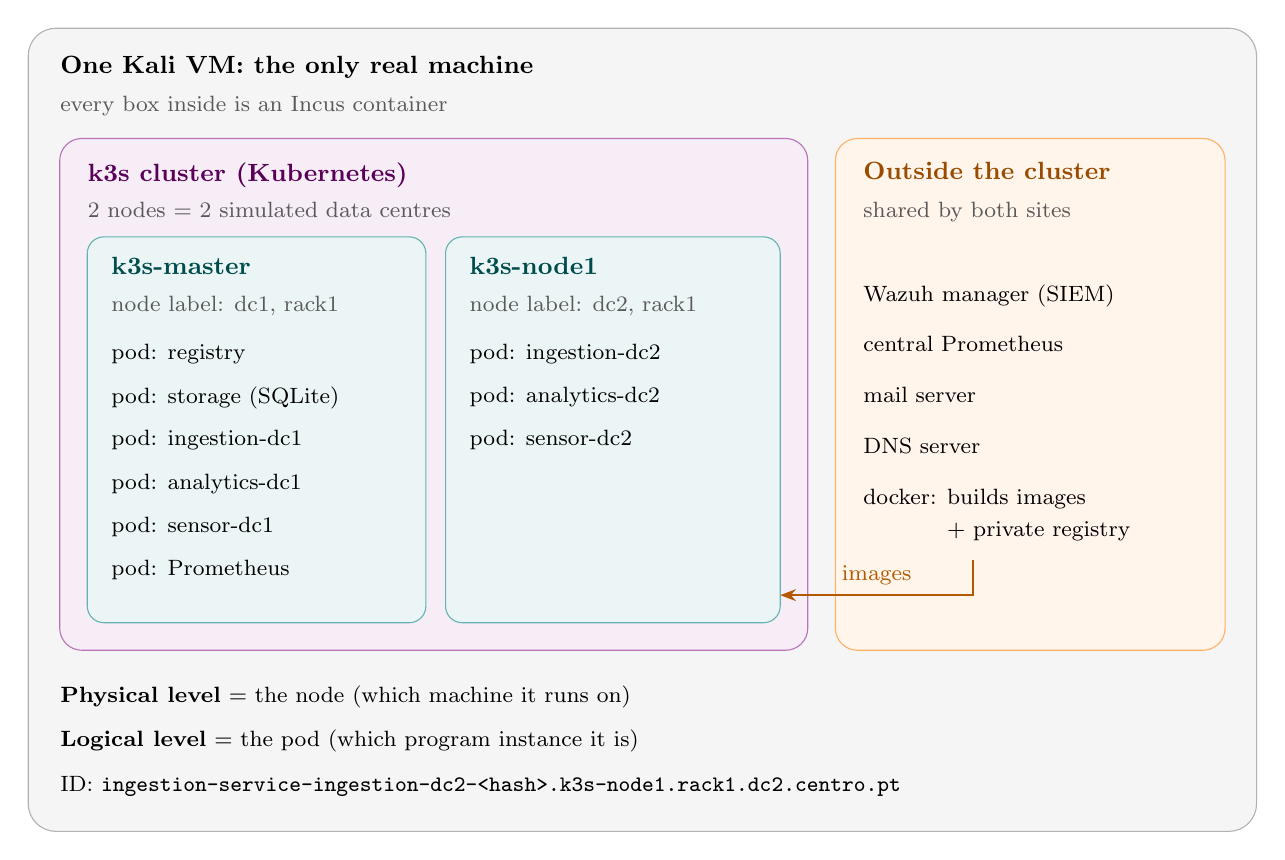
\begin{tikzpicture}[
  font=\small,
  title/.style={font=\small\bfseries, anchor=north west, inner sep=0pt},
  sub/.style={font=\footnotesize, anchor=north west, inner sep=0pt, text=black!65},
  item/.style={font=\footnotesize, anchor=north west, inner sep=0pt},
]
% one real machine
\draw[rounded corners=10pt, fill=gray!8, draw=gray!60] (0,0) rectangle (15.6,10.2);
\node[title] at (0.4,9.85) {One Kali VM: the only real machine};
\node[sub]   at (0.4,9.35) {every box inside is an Incus container};

% k3s cluster
\draw[rounded corners=8pt, fill=violet!7, draw=violet!55] (0.4,2.3) rectangle (9.9,8.8);
\node[title, text=violet!70!black] at (0.75,8.5) {k3s cluster (Kubernetes)};
\node[sub] at (0.75,8.0) {2 nodes = 2 simulated data centres};

% node dc1
\draw[rounded corners=6pt, fill=teal!8, draw=teal!60] (0.75,2.65) rectangle (5.05,7.55);
\node[title, text=teal!60!black] at (1.05,7.3) {k3s-master};
\node[sub] at (1.05,6.8) {node label: dc1, rack1};
\foreach \t [count=\i] in {registry, storage (SQLite), ingestion-dc1, analytics-dc1, sensor-dc1, Prometheus}
  \node[item] at (1.05,6.75-0.55*\i) {pod: \t};

% node dc2
\draw[rounded corners=6pt, fill=teal!8, draw=teal!60] (5.3,2.65) rectangle (9.55,7.55);
\node[title, text=teal!60!black] at (5.6,7.3) {k3s-node1};
\node[sub] at (5.6,6.8) {node label: dc2, rack1};
\foreach \t [count=\i] in {ingestion-dc2, analytics-dc2, sensor-dc2}
  \node[item] at (5.6,6.75-0.55*\i) {pod: \t};

% outside the cluster
\draw[rounded corners=8pt, fill=orange!8, draw=orange!60] (10.25,2.3) rectangle (15.2,8.8);
\node[title, text=orange!60!black] at (10.6,8.5) {Outside the cluster};
\node[sub] at (10.6,8.0) {shared by both sites};
\foreach \t [count=\i] in {Wazuh manager (SIEM), central Prometheus, mail server, DNS server, docker: builds images}
  \node[item] at (10.6,7.6-0.65*\i) {\t};
\node[item] at (10.6,3.95) {\phantom{docker: }+ private registry};

% images are pulled by the nodes
\draw[-{Stealth[length=2mm]}, thick, orange!70!black] (12.0,3.45) |- (9.55,3.0)
  node[pos=0.75, above, font=\footnotesize] {images};

% reading key
\node[item] at (0.4,1.85) {\textbf{Physical level} = the node (which machine it runs on)};
\node[item] at (0.4,1.3)  {\textbf{Logical level} = the pod (which program instance it is)};
\node[item] at (0.4,0.7)  {ID: \texttt{ingestion-service-ingestion-dc2-<hash>.k3s-node1.rack1.dc2.centro.pt}};
\end{tikzpicture}
}
\caption{Where every part runs. The only physical machine is one VM; every box inside it is an
Incus container. Two of them form the k3s cluster, and each node is labelled as a data centre. The
node is the physical level of an ID and the pod the logical level.}
\label{fig:layers}
\end{figure}

Two k3s nodes run as privileged Incus containers on
one VM; each node \emph{is} a data centre: \code{k3s-master} is \code{dc1} and \code{k3s-node1} is
\code{dc2}, both in \code{rack1}, region \code{centro}, country \code{pt} (node labels
\code{ssle.dc}, \code{ssle.rack}). Ingestion, analytics and the sensor run once per location, as one
Deployment each pinned with a \code{nodeSelector}; the registry, storage (one replica, persistent
volume) and the in-cluster Prometheus run in dc1. Images are built in a separate container and
pulled from a private registry, tagged with the git commit. The Wazuh manager, the central
Prometheus, the mail server and the DNS server run outside the cluster on the same host.

\begin{figure}[ht]
\centering
\resizebox{\textwidth}{!}{% Figure 1: deployment on k3s (main platform) with trust boundaries.
% Source facts: FACTS.md sections 2-6 (k8s/ssle.yaml, k3s/README.md, k3s/setup-cluster.sh).
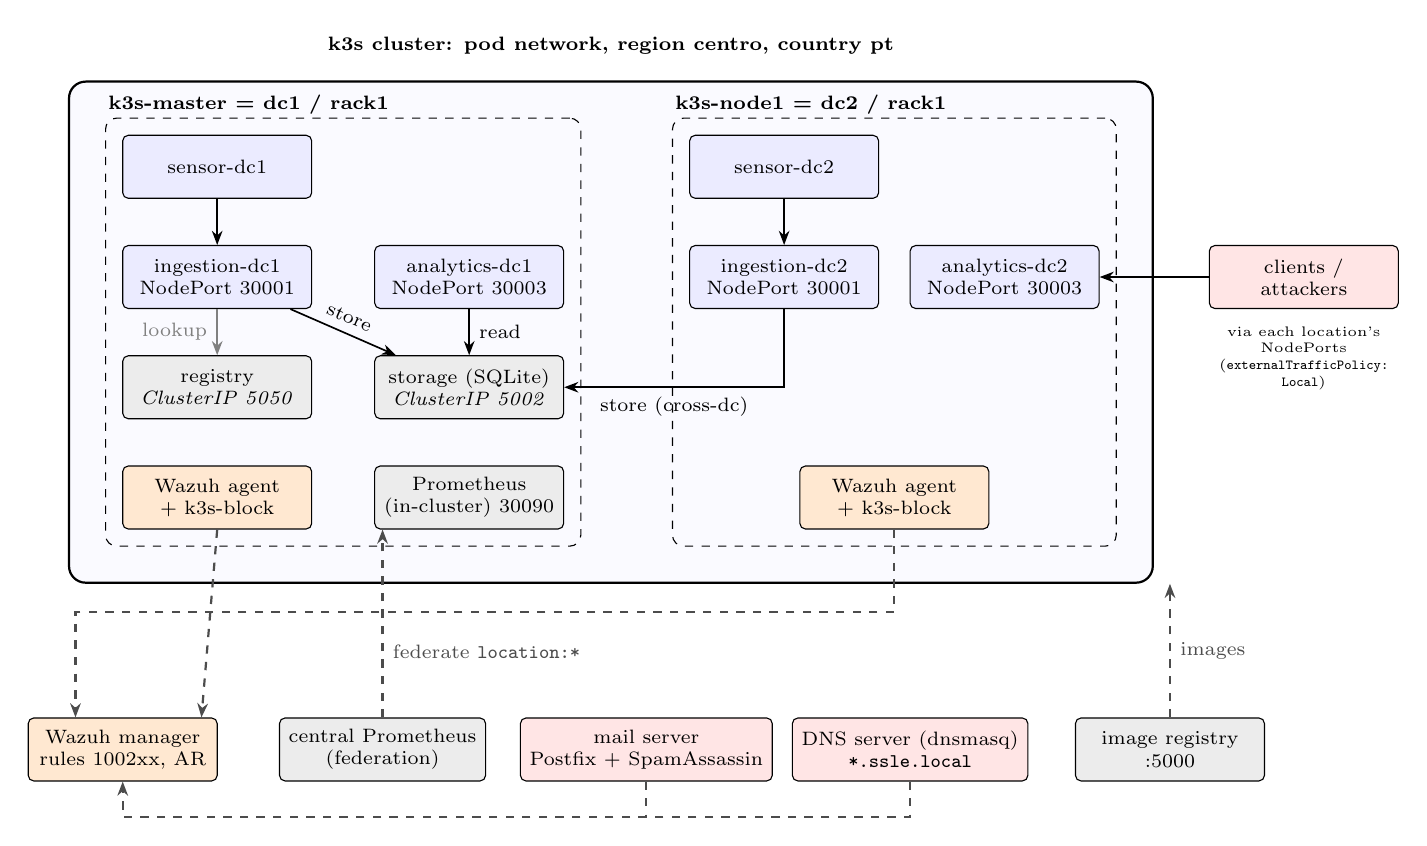
\begin{tikzpicture}[
  font=\scriptsize,
  svc/.style={draw, rounded corners=2pt, fill=blue!8, minimum width=24mm, minimum height=8mm, align=center},
  int/.style={svc, fill=gray!15},
  sec/.style={svc, fill=orange!18},
  ext/.style={svc, fill=red!10},
  flow/.style={-{Stealth[length=1.8mm]}, semithick},
  mon/.style={-{Stealth[length=1.8mm]}, dashed, thick, gray!60!black},
  bound/.style={draw, dashed, rounded corners=4pt, inner sep=6pt},
  lbl/.style={font=\scriptsize\bfseries, anchor=south west, inner sep=1pt}
]
% ---------------- node k3s-master = dc1
\node[svc] (sen1) at (1.4,3.0)  {sensor-dc1};
\node[svc] (ing1) at (1.4,1.6)  {ingestion-dc1\\NodePort 30001};
\node[svc] (ana1) at (4.6,1.6)  {analytics-dc1\\NodePort 30003};
\node[int] (reg)  at (1.4,0.2)  {registry\\\textit{ClusterIP 5050}};
\node[int] (sto)  at (4.6,0.2)  {storage (SQLite)\\\textit{ClusterIP 5002}};
\node[sec] (ag1)  at (1.4,-1.2) {Wazuh agent\\+ k3s-block};
\node[int] (pin)  at (4.6,-1.2) {Prometheus\\(in-cluster) 30090};
\node[bound, fit=(sen1)(ana1)(ag1)(pin)] (n1) {};
\node[lbl] at (n1.north west) {k3s-master = dc1 / rack1};

% ---------------- node k3s-node1 = dc2
\node[svc] (sen2) at (8.6,3.0)  {sensor-dc2};
\node[svc] (ing2) at (8.6,1.6)  {ingestion-dc2\\NodePort 30001};
\node[svc] (ana2) at (11.4,1.6) {analytics-dc2\\NodePort 30003};
\node[sec] (ag2)  at (10.0,-1.2) {Wazuh agent\\+ k3s-block};
\node[bound, fit=(sen2)(ana2)(ag2)] (n2) {};
\node[lbl] at (n2.north west) {k3s-node1 = dc2 / rack1};

\begin{scope}[on background layer]
  \node[draw, thick, rounded corners=6pt, fill=blue!2, inner sep=13pt, fit=(n1)(n2)] (cl) {};
\end{scope}
\node[font=\scriptsize\bfseries, anchor=south] at ([yshift=6pt]cl.north)
  {k3s cluster: pod network, region centro, country pt};

% ---------------- outside the cluster (same Incus host, lab network)
\node[sec] (wz)   at (0.2,-4.4)  {Wazuh manager\\rules 1002xx, AR};
\node[int] (pc)   at (3.5,-4.4)  {central Prometheus\\(federation)};
\node[ext] (mail) at (6.85,-4.4)  {mail server\\Postfix + SpamAssassin};
\node[ext] (dns)  at (10.2,-4.4)  {DNS server (dnsmasq)\\\code{*.ssle.local}};
\node[int] (dreg) at (13.5,-4.4) {image registry\\:5000};
\node[ext] (cli)  at (15.2,1.6)  {clients /\\attackers};

% ---------------- data flows
\draw[flow] (sen1) -- (ing1);
\draw[flow] (ing1) -- (sto) node[midway, above, sloped] {store};
\draw[flow] (ana1) -- (sto) node[midway, right] {read};
\draw[flow, gray] (ing1) -- (reg) node[midway, left] {lookup};
\draw[flow] (sen2) -- (ing2);
\draw[flow] (ing2.south) |- (sto.east) node[pos=0.75, below] {store (cross-dc)};
\draw[flow] (cli) -- (ana2);
\node[font=\tiny, align=center, below=1mm of cli] {via each location's\\NodePorts\\(\code{externalTrafficPolicy:}\\\code{Local})};

% ---------------- monitoring and security
\draw[mon] (pc.north) -- (pc.north |- pin.south) node[pos=0.35, right] {federate \code{location:*}};
\draw[mon] (ag1.south) -- ([xshift=10mm]wz.north);
\draw[mon] (ag2.south) -- ++(0,-1.05) -| ([xshift=-6mm]wz.north);
\draw[mon] (dns.south) -- ++(0,-0.45) -| (wz.south);
\draw[dashed, thick, gray!60!black] (mail.south) -- ++(0,-0.45);
\draw[mon] (dreg.north) -- (dreg.north |- cl.south) node[pos=0.5, right] {images};
\end{tikzpicture}
}
\caption{Main deployment on k3s: each node is a data centre. Grey services are internal
(ClusterIP), blue ones are published on NodePorts, dashed lines are monitoring and security
traffic.}
\label{fig:arch}
\end{figure}

The baseline deployment uses one Incus container per service with a systemd unit; the location
is given by environment variables. All tests and evidence exist for both platforms
(Section~\ref{sec:eval}), and the comparison is itself informative: three of the problems reported
in Section~\ref{sec:threats} only appeared on Kubernetes.

\subsection{Identification and registration of elements}
\label{sec:naming}

Every instance builds its ID from five location levels, most specific first, like a DNS
name~\cite{rfc1034}:
\[
\underbrace{\code{ingestion-service-ingestion-dc2-<hash>}}_{\text{service-instance (logical)}}.
\underbrace{\code{k3s-node1}}_{\text{node (physical)}}.\code{rack1}.\code{dc2}.\code{centro}.\code{pt}
\]
The node level is the machine that runs the element and the instance level is the logical element
on it: on Kubernetes they come from \code{spec.nodeName} and the pod name (downward API); on Incus
from the host name and an instance number (Figure~\ref{fig:idtree}). Dots inside a level are
replaced, so a label can never fake another level.

\begin{figure}[ht]
\centering
\resizebox{0.85\textwidth}{!}{% Figure 2: naming hierarchy and the k3s mapping. Source: common.py, k8s/ssle.yaml, FACTS.md section 3.
\begin{forest}
  for tree={font=\scriptsize, draw, rounded corners=2pt, align=center, l sep=4mm, s sep=2mm,
            edge={-{Stealth[length=1.3mm]}}, fill=blue!5}
  [{country\\\code{pt}}
    [{region\\\code{centro}}
      [{dc\\\code{dc1}\\(k3s node label)}
        [{rack\\\code{rack1}}
          [{node\\\code{k3s-master}\\(\code{spec.nodeName})}
            [{instance\\\code{storage-<pod>}}, fill=orange!15]
            [{instance\\\code{ingestion-dc1-<pod>}}, fill=orange!15]
          ]
        ]
      ]
      [{dc\\\code{dc2}}
        [{rack\\\code{rack1}}
          [{node\\\code{k3s-node1}}
            [{instance\\\code{ingestion-dc2-<pod>}}, fill=orange!15]
          ]
        ]
      ]
    ]
  ]
\end{forest}
}
\caption{Location hierarchy of the IDs. Orange leaves are the logical elements (pods); the node
level is the physical machine.}
\label{fig:idtree}
\end{figure}

Registration is decentralised: each instance posts \code{\{name, url, id, location\}} to the
registry every 10~s. The call is an idempotent upsert, so it doubles as a heartbeat and recovers
automatically when the registry restarts. On Kubernetes each pod registers its own pod IP; with the
Service address all replicas collapsed into one entry, a problem found and fixed during development. The registry checks
every instance's \code{/health} every 10~s and removes it after two consecutive failures. Queries
can be filtered by any level (\code{/services?dc=dc2}), and \code{/tree} returns instance counts per
country, region, dc, rack and node.

\subsection{Geographic location and delegation of responsibilities}

Location is used, not only recorded:
\begin{itemize}
  \item \textbf{Discovery prefers the closest instance.} A service first asks for instances in its own
        location up to a configurable scope (default: same dc), then any location, then a static
        fallback. The dc2 sensor therefore feeds the dc2 ingestion pod, as verified
        (Section~\ref{sec:eval}).
  \item \textbf{Each location serves its own clients.} The NodePorts use
        \code{externalTrafficPolicy: Local}, so a node only forwards to its own pods and keeps the
        client's source address~\cite{k8s_sourceip}, which the SIEM needs to block it.
  \item \textbf{Monitoring is delegated per site.} The in-cluster Prometheus scrapes the local pods;
        the central one only federates per-location aggregates and alerts.
  \item \textbf{Security enforcement is delegated per node.} One Wazuh agent per k3s node reads the
        logs of every pod on that node and executes the active responses locally; the manager only
        decides.
\end{itemize}

\subsection{Monitoring by location with optimised bandwidth}

Recording rules join every metric with \metric{service\_info} and sum it by country, region and dc:
\metric{location:http\_requests:rate1m}, \metric{location:http\_errors:rate1m},
\metric{location:http\_request\_duration\_seconds:p95} and \metric{location:instances:count}. The
central Prometheus federates only \code{\{\_\_name\_\_=\textasciitilde"location:.+"\}} (plus
\code{ALERTS}), following the hierarchical federation pattern~\cite{prometheus_federation}. Its
traffic grows with the number of locations, not with the number of pods; the measured saving is in
Section~\ref{sec:eval}.

\subsection{Locating the source of an event}

Because the same ID appears in the registry, in \metric{service\_info}, in every access-log line
and, at node level, in the Wazuh agent name (\code{k3s-node-01.k3s-node1.rack1.dc2.centro.pt}), any
event can be placed without a lookup table: a Wazuh alert names the node and carries the pod's full
ID in \code{data.id}; a Prometheus alert can be joined with \metric{service\_info} to get the
location. For example, the alerts of the DoS test identify both the attacker (\code{srcip}) and the
attacked pod in dc1 (Section~\ref{sec:threats}).

\subsection{Exposure and trust boundaries}

Only ingestion and analytics are reachable from outside the cluster (NodePorts 30001/30003). The
registry and storage are ClusterIP services: the registry has no authentication, so it must never
be exposed. Pods have CPU and memory limits (500m, 256~MiB) and readiness and liveness probes, which
both restart failed pods and cap what a flood can take from a node. The trust boundaries are
therefore: the lab network (clients, attackers, mail, DNS), the node (NodePorts, agent, firewall),
and the pod network (internal services, trusted by the SIEM rules, see
Section~\ref{sec:threats}). The k3s nodes run as \emph{privileged} containers, which is part of the
attack surface analysed next.

\section{Risk Management and Mitigation}
\label{sec:risk}

\subsection{Attack surface}

Table~\ref{tab:surface} lists every entry point of the deployment in Figure~\ref{fig:arch}, who can
reach it, the threat it enables and the control we have. Digital surface dominates: there are no
user accounts and the physical surface is a single host.

\begin{table}[ht]
\centering\small
\caption{Attack surface of the k3s deployment.}
\label{tab:surface}
\begin{tabularx}{\textwidth}{@{}>{\raggedright}p{3.3cm} >{\raggedright}p{2.1cm} >{\raggedright}X >{\raggedright\arraybackslash}X@{}}
\toprule
Entry point & Reachable from & Threat & Control in place \\
\midrule
ingestion / analytics NodePorts & lab network & HTTP flood; forged readings & Wazuh 100210 + k3s-block; Prometheus load alerts; pod limits; input validation \\
registry API (no auth) & pod network only & fake or hijacked registrations (discovery poisoning) & ClusterIP only; health checks remove dead entries; \emph{no authentication} \\
storage API & pod network only & data tampering, read-heavy load & ClusterIP only; single writer \\
SMTP (mail server) & lab network & spam, mail flood, open relay & SpamAssassin + hold queue; 100222 + firewall-drop; relay restrictions \\
DNS zone file & DNS host & redirection of service names & real-time FIM + restore-dns \\
DNS resolution path & lab network & cache poisoning, rogue resolver & \emph{none} \\
k3s nodes (privileged containers) & host & container escape = host compromise & \emph{none}; documented limitation \\
Image registry (plain HTTP) & lab network & image tampering & lab only, \emph{no TLS or signing} \\
Prometheus UI/API (9090, NodePort 30090) & lab network & reading the topology; spotting the thresholds & \emph{none}: no authentication \\
Wazuh dashboard (443) & lab network & blinding or misleading the defender & login page; API (55000) and indexer (9200) not reachable \\
\bottomrule
\end{tabularx}
\end{table}

\subsection{Attack and defense tree}

Figure~\ref{fig:adtree} refines the attacker goal \emph{disrupt or subvert the temperature service}
into the attacks we considered, with our countermeasures attached as defence nodes, in the notation
of attack--defense trees~\cite{kordy2010adtrees}. All children are OR-refinements: each leaf alone
reaches its parent goal. Grey nodes mark attacks for which we have no defence; they are the
limitations discussed in Section~\ref{sec:concl}. The three threats of Section~\ref{sec:threats}
correspond to the DoS, DNS and junk-email branches.

\begin{figure}[ht]
\centering
\resizebox{\textwidth}{!}{% Figure 3: attack-defense tree (Kordy et al. notation: attacks = red ellipses, defences = green
% boxes on dotted edges; grey = no defence in our system). Every defence is an element of the repo
% (FACTS.md sections 4-7); every "no defence" leaf is a documented limitation (FACTS.md section 10).
\begin{forest}
  for tree={font=\scriptsize, align=center, grow'=east, l sep=7mm, s sep=1.5mm, inner sep=2pt,
            child anchor=west, parent anchor=east, anchor=west},
  att/.style={ellipse, draw=red!70!black, fill=red!8},
  dfn/.style={rectangle, draw=green!50!black, fill=green!10, edge={dotted, thick}},
  gap/.style={rectangle, draw=gray, fill=gray!15, edge={dotted, thick}, font=\scriptsize\itshape},
  [{Disrupt or subvert\\the temperature service}, att
    [{Deny service\\(DoS)}, att
      [{HTTP flood from\\few sources}, att
        [{100210 +\\k3s-block 60\,s}, dfn]
        [{Prometheus rate/\\latency alerts}, dfn]
      ]
      [{Distributed flood\\below 15 req/10\,s\\per source}, att
        [{no automatic\\response}, gap]
      ]
      [{Flood from a\\compromised pod}, att
        [{exempted by\\100209}, gap]
      ]
    ]
    [{Redirect clients\\(DNS hijack)}, att
      [{Tamper with\\zone file}, att
        [{FIM 550$\to$100230\\+ restore-dns}, dfn]
      ]
      [{Cache poisoning /\\rogue DNS}, att
        [{not detected\\(DNSSEC: future)}, gap]
      ]
    ]
    [{Poison service\\discovery}, att
      [{Register fake\\instance}, att
        [{registry only\\ClusterIP}, dfn]
        [{no authentication}, gap]
      ]
    ]
    [{Junk email}, att
      [{Spam content}, att
        [{SpamAssassin $\to$\\hold queue}, dfn]
      ]
      [{Mail flood\\one source}, att
        [{100222 +\\firewall-drop}, dfn]
      ]
      [{Open relay\\abuse}, att
        [{relay\\restrictions}, dfn]
      ]
    ]
    [{Take over\\the host}, att
      [{Escape the\\privileged k3s\\container}, att
        [{no control}, gap]
      ]
    ]
  ]
\end{forest}
}
\caption{Attack--defense tree. Red ellipses: attacks; green boxes: our defences; grey boxes:
no effective defence in the current system.}
\label{fig:adtree}
\end{figure}

The tree makes two priorities visible. First, the DoS defence covers only one of three ways to deny
service; the other two (many sources, a compromised pod) are only \emph{seen} by Prometheus.
Second, the registry is the most valuable unauthenticated asset: a fake registration redirects
traffic exactly like a DNS hijack, but is invisible to file-integrity monitoring.

\subsection{Large-scale monitoring strategy}

Prometheus scrapes every instance every 5~s. In the cluster, pods are discovered through the
Kubernetes API and relabelled to the same job names as on Incus (\code{ssle-registry},
\code{ssle-ingestion}, \dots), so one rule file serves both platforms. The rules have three groups:

\begin{itemize}
  \item \textbf{Load anomalies} (\code{ssle-ddos-alerts}, every 5~s): request rate above 5~req/s
        per job, p95 latency above 50~ms, and more than 3 requests in flight.
  \item \textbf{Correlation and root cause} (\code{ssle-root-cause}): each alert is labelled
        \code or \code{kind=root-cause} and names a \code{root\_cause}. For example,
        \code{SSLERootCauseStorageDown} fires only when ingestion or analytics report storage errors
        \emph{and} storage itself is down, while \code{SSLERootCauseStorageUnreachable} blames the
        network or discovery when storage is up but unreachable, unless a request flood explains the
        errors. \code{SSLERootCauseRequestFlood} combines high latency and high rate on the same job
        and points the operator to Wazuh rule \rid{100210} for the source addresses.
  \item \textbf{Per-location aggregates} (\code{ssle-location-aggregates}), used for federation
        (Section~\ref{sec:arch}).
\end{itemize}

Two rules were changed after the tests proved them wrong: during the DoS test the
\emph{unreachable} rule blamed the network for timeouts caused by an overloaded storage, so it now
requires the errors to persist and excludes floods; and on Kubernetes a pod scaled to zero has no
\code{up} series at all, so every rule that checks \code{up} uses \code{or vector(0)}.

\subsection{Fault management (FCAPS) and the security gap}

Figure~\ref{fig:fcaps} maps the FCAPS fault-management workflow~\cite{itu2000m3400} to our tools.
Prometheus covers the classic part: it \emph{detects} anomalies, the hierarchical ID
\emph{isolates} the element, the root-cause rules \emph{correlate} symptoms, the registry and
Kubernetes \emph{resolve} failed instances, and each test produces the \emph{post-mortem}. The
root-cause test of Section~\ref{sec:eval} exercises this chain end to end.

\begin{figure}[ht]
\centering
\resizebox{\textwidth}{!}{% Figure 4: FCAPS fault-management workflow mapped to our tooling (FACTS.md sections 5, 6, 8, 9).
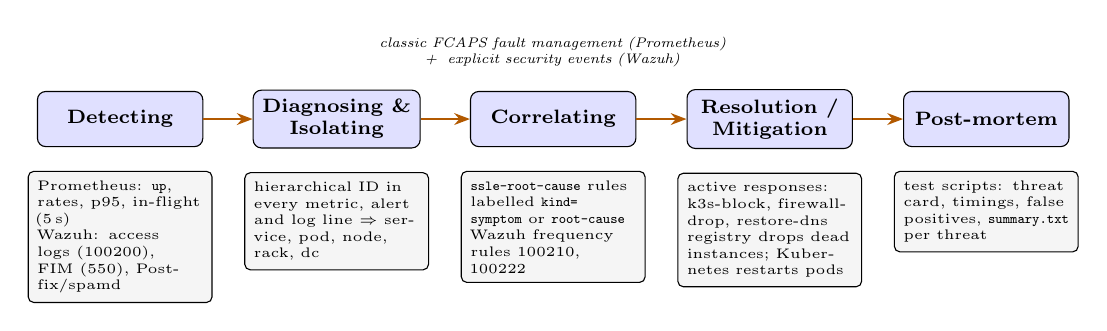
\begin{tikzpicture}[
  font=\scriptsize,
  stage/.style={draw, rounded corners=3pt, fill=blue!12, minimum width=21mm, minimum height=7mm, align=center, font=\scriptsize\bfseries},
  tool/.style={draw, rounded corners=2pt, fill=gray!8, text width=21mm, align=left, font=\tiny},
  arr/.style={-{Stealth[length=2mm]}, thick, orange!70!black}
]
\node[stage] (d) at (0,0)     {Detecting};
\node[stage] (i) at (2.75,0)  {Diagnosing \&\\Isolating};
\node[stage] (c) at (5.5,0)   {Correlating};
\node[stage] (r) at (8.25,0)  {Resolution /\\Mitigation};
\node[stage] (p) at (11,0)    {Post-mortem};
\foreach \a/\b in {d/i,i/c,c/r,r/p} \draw[arr] (\a) -- (\b);

\node[tool, below=3mm of d] {Prometheus: \code{up}, rates, p95, in-flight (5\,s)\\Wazuh: access logs (100200), FIM (550), Postfix/spamd};
\node[tool, below=3mm of i] {hierarchical ID in every metric, alert and log line $\Rightarrow$ service, pod, node, rack, dc};
\node[tool, below=3mm of c] {\code{ssle-root-cause} rules labelled \code{kind=}\\\code{symptom} or \code{root-cause}\\Wazuh frequency rules 100210, 100222};
\node[tool, below=3mm of r] {active responses: k3s-block, firewall-drop, restore-dns\\registry drops dead instances; Kubernetes restarts pods};
\node[tool, below=3mm of p] {test scripts: threat card, timings, false positives, \code{summary.txt} per threat};

\node[font=\tiny\itshape, align=center, text width=60mm] at (5.5,0.85)
  {classic FCAPS fault management (Prometheus) \;+\; explicit security events (Wazuh)};
\end{tikzpicture}
}
\caption{FCAPS fault-management workflow and the tool that implements each step.}
\label{fig:fcaps}
\end{figure}

FCAPS fault management does not deal with explicit security events: from Prometheus' point of view a
DNS hijack is not a fault at all (every service is up and answering), and a flood is only "high
load". The SIEM closes this gap. Wazuh receives the same access logs plus file-integrity and mail
events, correlates them with frequency rules (\rid{100210}, \rid{100222}) and triggers active
responses. The two systems are linked by the common ID and by cross-references: the Prometheus flood
root cause points to the Wazuh rule, and Wazuh's HTTP~5xx events (\rid{100201}) from each service
are the security-side view of the same symptoms the root-cause rules correlate.

\section{Approach to the Three Threats}
\label{sec:threats}

Three threats were chosen from the syllabus: \emph{massive denial-of-service disruptions},
\emph{junk email} and \emph{route and signal hijacking} (as DNS hijacking).
Table~\ref{tab:threats} summarises detection, response and the measured result on the main (k3s)
platform. Each proof of concept is an automated script that prints a threat card, runs the attack
from separate containers, checks detection, response, false positives and recovery, and stores the
raw evidence (alert JSON, firewall rules, logs, Prometheus queries). Every test passed on both
platforms: DoS 17/17 checks, junk email 18/18, DNS 10/10.

\begin{table}[ht]
\centering\small
\caption{Threats, detection, action-response and result on k3s.}
\label{tab:threats}
\begin{tabularx}{\textwidth}{@{}l Y Y Y@{}}
\toprule
Threat & Detection & Action-response & Result (k3s) \\
\midrule
HTTP flood (DoS) & Wazuh \rid{100210}: 15 requests in 10~s from one source; Prometheus rate, p95, in-flight alerts & \code{k3s-block}: drop the source in \code{raw/PREROUTING} on the node, 60~s & alert 2.2~s, blocked 2.8/2.9~s after start; legit client 91\%$\to$100\% \\
Junk email & \rid{100220} (spam), \rid{100223} (quarantined), \rid{100222}: 10 mails in 30~s from one source & spam held by Postfix; flood source \code{firewall-drop} 60~s; relay refused & spam not delivered; flood blocked 2.8~s; no false positive \\
DNS hijacking & FIM real time: \rid{550}$\to$\rid{100230} on the zone file & \code{restore-dns}: restore golden zone, restart dnsmasq & alert 0.1~s, restored 0.2~s; 0~s exposure seen \\
\bottomrule
\end{tabularx}
\end{table}

% ------------------------------------------------------------------------------------------
\subsection{Massive denial of service (HTTP flood)}

\paragraph{Description.}
An attacker sends far more requests than a service can handle, so legitimate requests are delayed
or dropped. At large scale the sources are many (botnets such as Mirai~\cite{antonakakis2017mirai});
the PoC uses a few sources, which is the case the defence targets.

\paragraph{Why it is relevant here.}
Analytics is the most exposed and most expensive endpoint: one \code{/stats?limit=1000} call makes
analytics query the registry and then read 1000 rows from storage. A flood on analytics is
therefore amplified onto storage, the single writer of the whole platform, and degrades ingestion
in every location.

\paragraph{How it can be exploited (PoC).}
Two attacker containers each run 20 concurrent workers against the dc1 analytics NodePort for
25~s, while a legitimate client sends about one request per second, below the detection threshold.
The test has four phases: (1) baseline, legitimate client alone; (2) unmitigated attack, with the
node's Wazuh agent stopped; (3) the same attack with detection and response; (4) recovery after the
block expires.

\paragraph{Monitoring and mitigation metrics.}
Every request produces a JSON access-log line that the node agent forwards (rule \rid{100200}).
Rule \rid{100210} fires when 15 such events from the same \code{srcip} arrive within 10~s.
Sources that are the platform's own services are excluded twice: Incus service addresses through
a CDB list, and the Kubernetes pod network through rule \rid{100209}, a level-0 child of
\rid{100200} that ends pod-to-pod requests before \rid{100210} counts them. On the Prometheus side,
\code{SSLEHighRequestRate}, \code{SSLEHighP95Latency} and \code{SSLEHighConcurrentRequests} watch
rate, latency and backlog per job, and \code{SSLERootCauseRequestFlood} combines them.

\paragraph{Action-response.}
Rule \rid{100210} triggers an active response on the agent that saw the flood, for 60~s. The stock
\code{firewall-drop} adds a DROP rule to the \code{INPUT} chain, which works for the Incus
containers but not for Kubernetes: NodePort traffic is translated by \code{kube-proxy} and then
\emph{forwarded} to the pod, so it never crosses \code{INPUT}. A custom script, \code{k3s-block},
implements the Wazuh active-response protocol and inserts the DROP into the \code{raw} table's
\code{PREROUTING} chain, before \code{kube-proxy}. Because of \code{externalTrafficPolicy: Local},
the node that sees the flood is the node the attacker uses, so blocking locally is enough.

\paragraph{Post-mortem.}
Table~\ref{tab:ddos} shows the legitimate client in each phase. On k3s the alert came 2.2~s after
the attack started and both attackers were blocked within 2.9~s; the legitimate client was never
flagged or blocked, both attackers were unblocked after 60~s, and Prometheus raised
\code{SSLEHighRequestRate} during the unmitigated phase.

\begin{table}[ht]
\centering\small
\caption{DoS test: legitimate client success rate and latency (p50 / p95, ms).}
\label{tab:ddos}
\begin{tabular}{@{}l cc cc@{}}
\toprule
 & \multicolumn{2}{c}{k3s (main)} & \multicolumn{2}{c}{Incus (baseline)} \\
\cmidrule(lr){2-3}\cmidrule(lr){4-5}
Phase & success & p50 / p95 & success & p50 / p95 \\
\midrule
1 baseline    & 100\% & 13 / 32     & 100\% & 11 / 14 \\
2 unmitigated & 91\%  & 900 / 1890  & 0\%   & 2003 / 2003 \\
3 mitigated   & 100\% & 12 / 22     & 77\%  & 10 / 2002 \\
\midrule
first \rid{100210} alert & \multicolumn{2}{c}{2.2~s} & \multicolumn{2}{c}{12.0~s} \\
attackers blocked after  & \multicolumn{2}{c}{2.8 / 2.9~s} & \multicolumn{2}{c}{13.8 / 12.4~s} \\
\bottomrule
\end{tabular}
\end{table}

What failed along the way is as instructive as the final result:
\begin{itemize}
  \item \textbf{Self-inflicted outage (Incus).} In the first automated run, storage and the registry
        saw analytics' fan-out calls as a flood and blocked analytics itself, so the defence took
        the service down. Internal sources are now excluded. The trade-off: a compromised internal
        service flooding another one is not blocked.
  \item \textbf{The same outage again on k3s.} Pod addresses change on every restart, so they
        cannot be listed. A \code{10.42.} prefix entry in the CDB list never matched, and a negated
        CIDR condition in the rule behaved as a positive match, so the analytics pod was blocked
        again. Rule \rid{100209} fixed it and keeps internal HTTP~5xx errors visible for root-cause
        correlation.
  \item \textbf{New pods were invisible to the SIEM.} Every new pod writes a new log file; the agent
        looked for new files only every 64~s, so the first minute of a new pod's traffic was never
        analysed. It now scans every 5~s.
  \item \textbf{Probes amplified overload.} With a 1~s liveness timeout, the kubelet killed pods
        that were slow but healthy (exit 137), which during a flood would restart the attacked pod.
        Liveness now tolerates about 60~s of silence; readiness still removes a struggling pod from
        the Service.
  \item \textbf{Symptoms differ by platform.} On Incus the flood made requests \emph{fail}; on k3s
        the pod limits kept the service answering, slowly (p50 900~ms). The check of the test was
        widened to accept a lower latency as evidence of mitigation.
  \item \textbf{An overloaded service delays its own detection.} Detection took 12.0~s on Incus and
        2.2~s on k3s, but the SIEM pipeline was fast on both: the first \rid{100210} alert came
        0.3~s (Incus) and 1.1~s (k3s) after the fifteenth logged request. The difference is that a
        request is logged when its response is sent. The saturated Incus analytics answered in
        about 2.3~s, so the 15 log lines the rule needs only existed about 9~s into the attack; the
        k3s pod answered in about 0.6~s.
\end{itemize}

Table~\ref{tab:ddos} shows single runs. Repeating the k3s test five times
(Section~\ref{sec:repeat}) gave the same picture in three runs, but in two the analytics pod was so
overloaded that detection took 17.4~s or did not happen.

\paragraph{Distributed flood (false negative).}
A per-source threshold cannot see an attack spread over many sources. This was tested with 40
source addresses (secondary addresses on the two attacker containers), each sending one request
per second, below the 1.5 per second that \rid{100210} needs, for 40~s against the same
endpoint; the generator skips missed slots instead of sending them in bursts. The service received
about 40~req/s in total (as measured by Prometheus) and Wazuh raised \emph{no} \rid{100210} alert
and added no block, while Prometheus fired \code{SSLEHighRequestRate} and
\code{SSLERootCauseRequestFlood} on analytics and storage. At this rate the legitimate client was
not seriously affected (p50 15~ms before, 13~ms during; p95 46 to 226~ms), but the attack was only
visible to Prometheus, which has no automatic response. A botnet would scale the same pattern.

% ------------------------------------------------------------------------------------------
\subsection{Junk email}

\paragraph{Description.}
Unsolicited bulk mail: unwanted content (advertising, phishing) and high-volume sending that
consumes the mail server's resources, plus abuse of the server as an open relay to send spam to
third parties.

\paragraph{Why it is relevant here.}
The mail server is the operators' channel (alerts, notifications) and is reachable from the lab
network. A flood fills its queues; an open relay would make the platform a spam source and get it
blacklisted; phishing reaching operators is the usual first step of an intrusion.

\paragraph{How it can be exploited (PoC).}
From an attacker container the test (1) sends a legitimate message from the legitimate client,
(2) sends a message containing the GTUBE string~\cite{spamassassin_gtube}, (3) tries to relay a
message to an outside domain, (4) opens 12 SMTP sessions in parallel, and (5) checks recovery after
the block.

\paragraph{Monitoring and mitigation metrics.}
Postfix passes every message through SpamAssassin (threshold 5.0; Bayes is enabled in the
configuration but has never been trained, so scores come from the rules alone). Rule
\rid{100220} matches \emph{spamd: identified spam}; \code{header\_checks} moves any message with
\code{X-Spam-Flag: YES} to the hold queue, and Postfix's log line becomes rule \rid{100223}. Rule
\rid{100221} marks each accepted message with its client address, and \rid{100222} fires on 10 of
them from the same source within 30~s. Relaying is refused for any client outside
\code{mynetworks} (localhost only).

\paragraph{Action-response.}
Two layers: the \emph{mail server} itself quarantines spam (hold queue, released by an operator)
and refuses relaying; \emph{Wazuh} responds to a flood (\rid{100222}) with \code{firewall-drop} of the
source on the mail container for 60~s. The spam alerts \rid{100220}/\rid{100223} are alert-only.

\paragraph{Post-mortem.}
On both platforms the legitimate message was delivered and scored clean; the GTUBE message was
flagged, quarantined and not delivered; the relay attempt was refused (\emph{Relay access
denied}). For the flood, the first \rid{100222} alert came 2.2~s after it started and the source was
blocked 2.8~s after it started on the k3s run (1.7~s and 2.0~s on the Incus run). The legitimate
sender was never blocked and could send during the block, and the attacker could connect again after
60~s. How many of the 12 flood messages got through is a race between the parallel sessions and the
block: 2 completed in the Incus run and all 12 in the k3s run. With a threshold of 10 messages, up
to about 10 messages from a new source are accepted before the block.

GTUBE only proves that the pipeline works. To measure detection, 500 spam and 500
legitimate (\emph{easy ham}) messages from the SpamAssassin public corpus (2003) were passed through the
production \code{spamd} (Table~\ref{tab:corpus}); Bayes auto-learning left no database behind. At the
configured threshold 70\% of the spam was caught and 10\% of the legitimate mail would have been
quarantined; lowering the threshold to 3.0 catches more spam but flags almost half of the
legitimate mail. The corpus is old, so its spam may miss current rules and its legitimate mail may
trip date-based ones; which rules caused the false positives was not analysed. Without Bayes
training and network tests, content filtering alone is weak, which is why the quarantine is
reviewed by an operator rather than deleting mail. Other limitations: a sender that rotates
addresses or stays under 10 messages per 30~s is not blocked.

\begin{table}[ht]
\centering\small
\caption{SpamAssassin on 500 spam + 500 legitimate messages (public corpus, untrained Bayes).}
\label{tab:corpus}
\begin{tabular}{@{}lcc@{}}
\toprule
Threshold & spam detected & legitimate flagged (false positive) \\
\midrule
5.0 (configured) & 349/500 (69.8\%) & 52/500 (10.4\%) \\
3.0 & 438/500 (87.6\%) & 226/500 (45.2\%) \\
\bottomrule
\end{tabular}
\end{table}

% ------------------------------------------------------------------------------------------
\subsection{Route and signal hijacking: DNS hijacking}

\paragraph{Description.}
The attacker changes the answer to a name lookup so that clients reach a machine of the attacker's
choice instead of the real service. This work considers tampering with the authoritative zone, the case
behind the 2019 DNS infrastructure hijacking campaigns~\cite{cisa2019ed1901}.

\paragraph{Why it is relevant here.}
Clients reach the platform by name: \code{ingestion.ssle.local} and \code{analytics.ssle.local}
point at the node that publishes the NodePorts. Redirecting \code{ingestion} sends every sensor
reading to the attacker (data theft and silent data loss) and lets it return fake answers, while
every service stays up and no fault alarm fires.

\paragraph{How it can be exploited (PoC).}
The test overwrites the zone file \code{/etc/dnsmasq-zones/ssle.hosts} so that
\code{ingestion.ssle.local} points to an attacker container, while a client resolves the name every
0.25~s. A control phase repeats the attack with the DNS host's Wazuh agent stopped.

\paragraph{Monitoring and mitigation metrics.}
The DNS host's agent monitors \code{/etc/dnsmasq-zones} with real-time file-integrity monitoring
(all checks). A change raises Wazuh rule \rid{550} (integrity checksum changed), and the custom rule
\rid{100230} (level 12) matches it for the zone file. The client's resolution timeline measures the
exposure window.

\paragraph{Action-response.}
\code{restore-dns} runs on the DNS host: it copies the golden zone over the live one and restarts
dnsmasq, but only if they differ, so its own restore does not trigger it again.

\paragraph{Post-mortem.}
\rid{100230} fired 0.1~s after the hijack and the zone was restored 0.2~s after it on the k3s run
(0.3~s on Incus). The client never received the attacker's address (exposure 0.00~s at a 0.25~s
sampling interval). Without Wazuh the hijack was still in place after 15~s. Limitations: only
tampering with the zone \emph{file} is detected, not cache poisoning, a rogue DNS or DHCP server or
on-path spoofing, for which DNSSEC~\cite{rfc4033} would be needed; clients may keep a bad answer
for its TTL; root on the DNS host could change the golden copy or stop the agent. Inside the cluster
the equivalent attack would target the CoreDNS configuration, which file monitoring does not see;
it would need Kubernetes audit logs in Wazuh.

\section{Evaluation of the Approaches and Scalability}
\label{sec:eval}

\subsection{Test setup}

All measurements come from the automated test scripts in the repository: single runs on 18
November 2026 (the numbers quoted in Section~\ref{sec:threats}) and repeated runs on 21 November
(Section~\ref{sec:repeat}).
Everything runs on one VM (4 vCPUs, 7.7~GiB RAM) as Incus containers: the two k3s nodes, the
Wazuh manager (4.14), the central Prometheus (2.53), the mail and DNS servers, and the load
generators. Locations are therefore \emph{logical}: dc1 and dc2 share the same CPU and disk, so
absolute numbers are lower bounds and the trends are what matters.

The scalability test uses three load-generator containers with 8 workers each, 20~s per phase, in
a closed loop (each worker sends its next request when the previous one returns). The Wazuh agents
are stopped during this test so the DoS rule does not block the load generators; it measures
capacity, not defence.

\subsection{Functional properties of the main deployment}

The cluster test checks every property of the architecture on k3s and passed 40/40 checks: both
nodes ready and labelled with their location; every Deployment available, each location's pods on
its own node, all images from the private registry; one registry entry per pod (pod addresses, both
dc1 and dc2) with the node name in the ID; readings accepted by the ingestion pod of each location;
the real client address in the pod's log; registry and storage not exposed; every service scraped
and the per-location aggregates federated centrally; both node agents active and a pod's access log
reaching the manager with the pod's ID; and self-healing: a deleted ingestion pod was replaced, the
new pod registered itself, and the health checker removed the old entry 15.8~s after the new one
registered.

\subsection{Horizontal scaling across locations}

Table~\ref{tab:scale} compares one instance (dc1) with two (dc1 and dc2) under the same load.

\begin{table}[ht]
\centering\small
\caption{Throughput and p95 latency with one and two instances.}
\label{tab:scale}
\begin{tabular}{@{}l rrr rr@{}}
\toprule
 & \multicolumn{3}{c}{throughput (req/s)} & \multicolumn{2}{c}{p95 (ms)} \\
\cmidrule(lr){2-4}\cmidrule(lr){5-6}
Service, platform & 1 inst. & 2 inst. & speed-up & 1 inst. & 2 inst. \\
\midrule
ingestion, k3s   & 85.8  & 114.8 & 1.34$\times$ & 426 & 475 \\
analytics, k3s   & 119.4 & 133.6 & 1.12$\times$ & 285 & 383 \\
ingestion, Incus & 189.9 & 184.3 & 0.97$\times$ & 199 & 540 \\
analytics, Incus & 194.3 & 207.9 & 1.07$\times$ & 175 & 234 \\
\bottomrule
\end{tabular}
\end{table}

Adding an instance helps little, and the reason is visible in the storage metrics: on Incus storage
wrote 198 readings/s with one ingestion instance and 184.7/s with two. Every write goes to one
SQLite storage, so a second ingestion instance only moves the bottleneck. Analytics only reads and
scales slightly better. Since both locations share one physical host, a second instance also
competes for the same CPU; these numbers cannot separate the two effects. During the repeated
runs analytics used up to 436 millicores of its 500-millicore limit and storage up to 350, so the
pods were close to their own CPU limits as well. Section~\ref{sec:repeat} shows how noisy these
measurements are.

\subsection{Registry growth}

The registry was filled with 0, 100, 500 and 2000 fake instances spread over 2 countries,
3 regions, 4 data centres and 5 racks (Figure~\ref{fig:registry}). On Incus, registration ran at
747--851 per second, and a filtered lookup stayed under 2~ms at the median (3.4~ms p95) with 2000
instances. The unfiltered \code{/services} response grows linearly to 404~kB, while a query for one
data centre returns 17~kB and for one rack 3.4~kB: filtering by location keeps discovery cost
proportional to the part of the system a client cares about. On k3s, where the benchmark runs
through the cluster network, 2000 instances gave 298 registrations/s and 4.1~ms (p50) / 38.7~ms
(p95) lookups.

\begin{figure}[ht]
\centering
% Figure 5: registry growth (Incus run, evidence/scale/3-registry.txt; FACTS.md section 9.6).
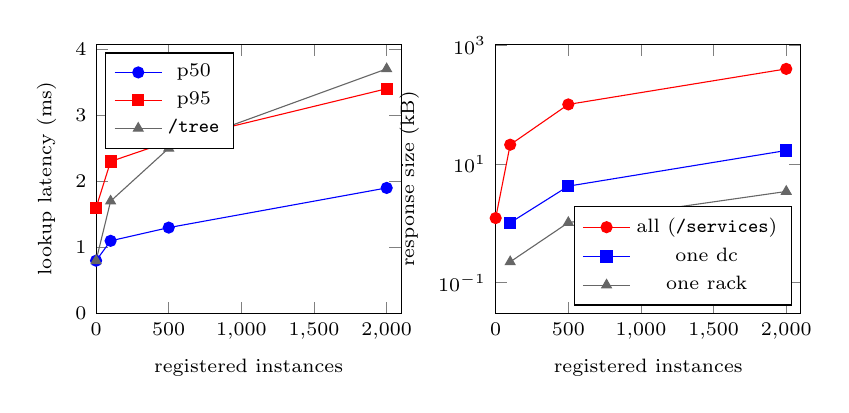
\begin{tikzpicture}
\begin{axis}[
  name=lat, width=0.45\textwidth, height=5cm,
  xlabel={registered instances}, ylabel={lookup latency (ms)},
  xmin=0, xmax=2100, ymin=0, legend pos=north west, legend style={font=\scriptsize},
  tick label style={font=\scriptsize}, label style={font=\scriptsize},
  scaled x ticks=false, xtick={0,500,1000,1500,2000}]
\addplot[mark=*, blue] coordinates {(0,0.8) (100,1.1) (500,1.3) (2000,1.9)};
\addlegendentry{p50}
\addplot[mark=square*, red] coordinates {(0,1.6) (100,2.3) (500,2.6) (2000,3.4)};
\addlegendentry{p95}
\addplot[mark=triangle*, black!60] coordinates {(0,0.8) (100,1.7) (500,2.5) (2000,3.7)};
\addlegendentry{\texttt{/tree}}
\end{axis}
\begin{axis}[
  at={(lat.east)}, anchor=west, xshift=12mm,
  width=0.45\textwidth, height=5cm,
  xlabel={registered instances}, ylabel={response size (kB)},
  ymode=log, ymin=0.03, xmin=0, xmax=2100, legend pos=south east, legend style={font=\scriptsize},
  tick label style={font=\scriptsize}, label style={font=\scriptsize},
  scaled x ticks=false, xtick={0,500,1000,1500,2000}]
\addplot[mark=*, red] coordinates {(0,1.226) (100,21.209) (500,101.473) (2000,403.593)};
\addlegendentry{all (\texttt{/services})}
\addplot[mark=square*, blue] coordinates {(100,1.024) (500,4.240) (2000,16.950)};
\addlegendentry{one dc}
\addplot[mark=triangle*, black!60] coordinates {(100,0.224) (500,1.028) (2000,3.449)};
\addlegendentry{one rack}
\end{axis}
\end{tikzpicture}

\caption{Registry with a growing number of instances (Incus run). Left: lookup latency and
\code{/tree}; right: response size of an unfiltered vs location-filtered query (log scale).}
\label{fig:registry}
\end{figure}

\subsection{Monitoring bandwidth by location}

One full scrape of an instance is 7--15~kB (registry 14.6~kB, storage 9.3~kB, ingestion 7.2~kB,
analytics 7.1~kB). A central Prometheus federating every raw series from the site Prometheus would
transfer 326.5~kB per scrape on Incus (10.8~kB gzip) and 403.6~kB on k3s; federating only the
\code{location:*} aggregates transfers 2.8~kB on Incus (0.4~kB gzip) and 2.9~kB on k3s, i.e.\
0.7\% of the raw federation. The per-location view still answers the operator's first question
(how many instances, how much traffic and errors, which latency in each data centre) and the
detail stays in the site Prometheus.

\subsection{Correlation and root cause}

Stopping storage produced several symptoms and one diagnosis (Table~\ref{tab:rootcause}). The
correlation rule named storage as root cause and did not blame the network, the registry dropped
the dead instance, and the alert cleared after recovery. The longer times on k3s are consistent with how
Kubernetes discovery works: a pod scaled to zero disappears from service discovery instead of reporting
\code{up == 0}, and its address stops answering, so each health check waits for its timeout.

\begin{table}[ht]
\centering\small
\caption{Root-cause test: storage stopped.}
\label{tab:rootcause}
\begin{tabular}{@{}l c c@{}}
\toprule
 & k3s & Incus \\
\midrule
\code{SSLERootCauseStorageDown} firing after & 43.4~s & 11.3~s \\
registry removed storage after & 54.1~s & 20.8~s \\
symptoms correlated (Prometheus alerts + Wazuh 5xx events) & 4 + 4 $\to$ 1 & 3 + 3 $\to$ 1 \\
alert cleared after restart & 7.1~s & 10.8~s \\
\bottomrule
\end{tabular}
\end{table}

\subsection{Repeated runs}
\label{sec:repeat}

Each k3s test was repeated five times back to back (scalability three times) to see how stable the
single-run numbers are (Table~\ref{tab:repeat}).

\begin{table}[ht]
\centering\small
\caption{Repeated runs on k3s (21 November): mean $\pm$ standard deviation and range.}
\label{tab:repeat}
\begin{tabular}{@{}l l r@{}}
\toprule
Test & quantity & mean $\pm$ sd (min--max), runs \\
\midrule
DNS hijack & alert after hijack & 0.12 $\pm$ 0.04~s (0.1--0.2), 5 \\
           & zone restored after & 0.28 $\pm$ 0.08~s (0.2--0.4), 5 \\
           & exposure seen by client & 0~s in all 5 \\
Junk email flood & first \rid{100222} alert & 1.8 $\pm$ 0.7~s (1.2--2.7), 5 \\
                 & source blocked after & 3.0 $\pm$ 2.5~s (1.5--7.3), 5 \\
Root cause & \code{SSLERootCauseStorageDown} firing & 40.9 $\pm$ 2.6~s (38--44), 5 \\
           & registry removed storage & 52.7 $\pm$ 2.2~s (49.6--54.9), 5 \\
           & alert cleared after restart & 5.3 $\pm$ 2.5~s (1.5--7.1), 5 \\
DoS & first \rid{100210} alert & 1.8, \emph{none}, 17.4, 1.6, 1.8~s (per run) \\
    & legitimate success, mitigated & 100, 0, 38, 100, 100\,\% (per run) \\
Scalability & ingestion speed-up (2 vs 1) & 0.37, 1.37, 1.27$\times$ (per run) \\
            & analytics speed-up & 5.66, 1.16, 1.22$\times$ (per run) \\
            & \code{location:*} share of raw federation & 0.71 $\pm$ 0.01\,\%, 3 \\
            & registry lookup with 2000 instances & p50 4.4 $\pm$ 0.6~ms, p95 47.5 $\pm$ 10.4~ms, 3 \\
\bottomrule
\end{tabular}
\end{table}

DNS restoration, the mail flood response, the root-cause diagnosis and the monitoring bandwidth
are stable. The DoS defence is not. In three of five runs the attackers were blocked within about
3~s and the legitimate client got 100\% of its requests through. In run~2 the analytics pod
completed \emph{no} request during the mitigated phase, so nothing was logged and Wazuh detected
nothing: the extreme case of the logging-on-completion weakness described in
Section~\ref{sec:threats}. Run~3 started while the service was still overloaded (its baseline
already failed), and detection took 17.4~s. The defence therefore depends on the attacked service
staying responsive enough to log the attack. The root-cause test also failed one of its own checks
in four runs because the previous run's symptom alert, computed over a one-minute window, had not
cleared yet; the diagnosis itself was correct in all five.

The scalability results vary too much to support a speed-up figure. Runs 2 and 3 agree (ingestion
1.37$\times$ and 1.27$\times$, analytics 1.16$\times$ and 1.22$\times$), but in run~1 the one-instance
analytics phase reached only 7.4~req/s, and at the end of that run the registry pod was killed by
its liveness probe (exit 137) after the 2000-instance benchmark, presumably because checking 2000 unreachable instances kept it
too busy to answer \code{/health} in time. The single-run speed-ups in
Table~\ref{tab:scale} should be read as indicative only.

\paragraph{Monitoring cost.} During the repeated scalability runs (samples every 5~s), the
in-cluster Prometheus used at most 44 millicores of CPU and 51--109~MiB of memory, with about 2\,200
active series; the central Prometheus container used 59--143~MiB. The Wazuh manager container used
2.0--2.6~GiB, by far the largest share of the monitoring and security stack on this host.

\subsection{SIEM throughput per node}

We wrote synthetic access-log lines on one k3s node at increasing rates for 30~s each and counted
how many became alerts at the manager and how late (log timestamp to alert timestamp). Each line
used a different source address, so no active response was triggered. Up to 500 lines/s every line
became an alert within about 2~s; above that the node's agent delivered at most about 590 events/s,
lost the rest and logged \emph{Agent buffer is full: Events may be lost}
(Table~\ref{tab:eps}). The cause is the agent's client buffer, configured at 500 events per second
with a 5000-event queue. Because one agent serves a whole node, a flood of more than about 500
logged requests per second on one node \emph{blinds the SIEM for every pod on that node}: the
first 15 requests still trigger \rid{100210}, but other events from the same node (for example
5xx errors from an unrelated pod) can be lost or arrive 11--15~s late. We did not measure the
manager's own limit, which a higher agent limit would expose.

\begin{table}[ht]
\centering\small
\caption{Wazuh pipeline from one k3s node: delivered alerts and latency per log rate (30~s each).}
\label{tab:eps}
\begin{tabular}{@{}rrrrrr@{}}
\toprule
lines/s & written & alerts & lost & p50 latency & p95 latency \\
\midrule
100  & 2\,884  & 2\,884  & 0\%    & 1.1~s  & 1.8~s \\
250  & 7\,499  & 7\,499  & 0\%    & 1.1~s  & 1.5~s \\
500  & 14\,999 & 14\,999 & 0\%    & 2.3~s  & 3.7~s \\
1000 & 29\,996 & 17\,777 & 40.7\% & 11.2~s & 12.1~s \\
2000 & 59\,992 & 16\,900 & 71.8\% & 11.5~s & 15.2~s \\
\bottomrule
\end{tabular}
\end{table}

\subsection{Scaling limits of each component}

\begin{itemize}
  \item \textbf{Storage} is a single SQLite writer: the measured bottleneck. Sharding by location or a
        replicated database is required before more ingestion instances help.
  \item \textbf{Registry} is a single in-memory process. Lookups stay fast, but the health checker
        pings every instance one after another (O($N$) per sweep, plus a 2~s timeout per dead
        instance), and unfiltered queries grow linearly. A registry per location, with the
        hierarchy delegated like DNS zones, would bound both.
  \item \textbf{Prometheus} is one server per site plus a central one; federation of aggregates keeps
        the central load proportional to the number of locations. At our size it is cheap (at most
        44 millicores and about 100~MiB for about 2\,200 series); its cost grows with the number of
        series, i.e.\ with instances and label combinations, which is why no client-controlled value
        is used as a label.
  \item \textbf{Wazuh} is a single manager. One agent per node instead of per pod keeps the number of
        agents proportional to machines, not pods, and avoids enrolling a new agent at every
        restart. The binding limit, however, is per agent (Table~\ref{tab:eps}).
  \item \textbf{Shared host.} All nodes share one disk: when free space fell below 5\%, the kubelet
        evicted every pod and blocked scheduling on both nodes. In a real multi-site deployment
        this failure would stay local to one site.
  \item \textbf{Operations.} After a reboot of the VM the Wazuh manager failed to start (its start-up
        timed out on the busy host) and nothing alerted on it: the SIEM was silently down until we
        noticed missing alerts. The stock service allows 45~s to start and never retries; we added a
        systemd override (5~min, restart on failure). Monitoring the SIEM itself (an \code{up}
        check on the manager) would still be needed to notice such a failure.
\end{itemize}

\section{Conclusions}
\label{sec:concl}

\paragraph{Findings and contributions.}
A single hierarchical name, used unchanged by the registry, the metrics, the SIEM and the logs, was
the most useful design decision: every alert in this report names the pod, node and data centre
involved without any lookup. The same name made location-aware discovery and per-location
monitoring cheap to add, and federating only per-location aggregates reduced the central monitoring
traffic to 0.7\% of a raw federation. Wazuh detected all three threats and responded automatically
on both platforms, with no false positive against the legitimate clients. Over five repeated runs a
tampered DNS zone was restored after 0.28~s on average and a mail flood was blocked after 3.0~s;
flood sources were blocked within about 3~s in three runs, but in the other two the attacked
service was too overloaded to log the requests the detection depends on. Prometheus' correlation rules reduced each storage failure to one root-cause
alert. Moving the platform to Kubernetes required changes that only showed up under attack: a
block that acts before \code{kube-proxy}, an exception for the pod network, faster discovery of new
pod logs, and gentler liveness probes.

\paragraph{Why the solution is not perfect.}
\begin{itemize}
  \item \textbf{Detection depends on the victim.} Requests are logged when they complete, so a
        service too overloaded to answer is also too overloaded to be protected: in one of five
        DoS runs nothing was detected at all.
  \item \textbf{Per-source thresholds.} Both flood rules count requests per source address. In the
        test, 40 sources at one request per second each produced no Wazuh alert at all; only
        Prometheus saw the flood, and nothing responds automatically.
  \item \textbf{The SIEM can be blinded.} Each node's agent forwards at most about 500 events per
        second; above that, events from every pod on the node are lost or delayed by more than
        10~s. A flood therefore also hides whatever else happens on the attacked node.
  \item \textbf{Trusted interior.} Internal sources are exempt from the flood rule to avoid a
        self-inflicted outage, so a compromised pod can flood its neighbours unchallenged.
  \item \textbf{Unauthenticated registry.} A fake registration would redirect traffic like a DNS
        hijack and is invisible to file-integrity monitoring.
  \item \textbf{Narrow DNS coverage.} Only tampering with the zone file is detected; cache
        poisoning, rogue resolvers, on-path spoofing and CoreDNS changes are not.
  \item \textbf{Weak content filtering.} With untrained Bayes, SpamAssassin caught 70\% of a public
        spam corpus and would have quarantined 10\% of legitimate mail.
  \item \textbf{Hand-written correlation.} Root-cause rules exist per dependency (storage,
        ingestion); new services need new rules.
  \item \textbf{Single points of failure and a single host.} One registry, one SQLite writer, one
        Wazuh manager, privileged k3s nodes, and all locations on one machine: the numbers are lower
        bounds, the scalability measurements are noisy (Section~\ref{sec:repeat}), and the root of
        the deployment is a single failure domain.
  \item \textbf{Defences can hurt.} Twice the DoS response blocked the platform's own service, and the liveness
        probes once killed healthy pods under load. Every response needs its own false-positive
        test.
\end{itemize}

\paragraph{Future work.}
The second project (attack tolerance) can build directly on these gaps: authenticated, replicated
registries per location with the hierarchy delegated like DNS zones; replicated or sharded
storage; distributed-flood detection that feeds Prometheus anomalies into Wazuh so they can trigger
responses (for example rate limiting per location rather than per source); Kubernetes audit logs
and network policies to cover CoreDNS tampering and pod-to-pod abuse; a dependency graph or
Alertmanager inhibition to generate root-cause rules; a Wazuh manager cluster; and repeated
measurements on separate physical hosts.


\section*{Use of AI tools}
\TODO{keep or delete}
AI assistance was used for drafting and wording support. The architecture, implementation,
experiments and analysis are the authors' own.

\bibliographystyle{plainnat}
\bibliography{references}

\appendix
\section{Reproducing the results}
\label{app:repro}

All code, configuration, test scripts and raw evidence are in the project repository:
\begin{center}\url{https://github.com/raquelmeira205/ssle_Proj1}\end{center}
\noindent All commands run on the Incus host from the repository root; \code{commands.md} documents every
option. Evidence is written to \code{evidence/k3s/<test>/} for the main platform and
\code{evidence/<test>/} for the Incus baseline.

\paragraph{Main platform (k3s).}
\begin{verbatim}
./k3s/setup-cluster.sh && ./apply-configs.sh pin && ./k3s/deploy.sh
./k3s/install-wazuh-node-agents.sh && PLATFORM=k3s ./apply-configs.sh
./test-k3s.sh                          # architecture, 40 checks
PLATFORM=k3s ./test-ddos.sh            # threat 1
PLATFORM=k3s ./test-spam.sh            # threat 2
PLATFORM=k3s ./test-dns.sh --control   # threat 3
PLATFORM=k3s ./test-rootcause.sh       # correlation / root cause
PLATFORM=k3s ./test-scale.sh           # scalability
\end{verbatim}

\paragraph{Baseline (Incus).}
\begin{verbatim}
./deploy-incus.sh && ./install-wazuh-agents.sh && ./apply-configs.sh
./test-incus.sh
./test-ddos.sh ; ./test-spam.sh ; ./test-dns.sh --control
./test-rootcause.sh ; ./test-scale.sh
\end{verbatim}

\paragraph{Where things are.}\mbox{}\\[2pt]
\noindent
\begin{tabularx}{\textwidth}{@{}l X@{}}
\code{common.py} & naming, registration, discovery, metrics, access log \\
\code{registry/}, \code{ingestion/}, \dots & the five services (one folder each) \\
\code{k8s/ssle.yaml}, \code{k8s/monitoring.yaml} & Kubernetes manifests, in-cluster Prometheus \\
\code{prometheus/ssle\_rules.yml} & load, root-cause and per-location rules \\
\code{wazuh/ssle-rules.xml} & Wazuh rules 100200--100230 \\
\code{wazuh/active-response/} & \code{k3s-block.py}, \code{restore-dns.sh} \\
\code{mail/}, \code{dns/} & Postfix/SpamAssassin hardening, DNS zone and golden copy \\
\code{evidence/} & raw evidence and \code{summary.txt} for every test \\
\end{tabularx}

\section{Evidence excerpts}
\label{app:evidence}

Short excerpts of the raw evidence of the k3s runs (\code{evidence/k3s/}). Lab addresses are
replaced by placeholders in angle brackets; nothing else is changed.

\paragraph{DoS: Wazuh alert and the block on the node} (\code{ddos/run.log},
\code{ddos/3-iptables-during-block.txt}). The agent name gives the node and location; the
\code{raw PREROUTING} rules are the ones added by \code{k3s-block}.
{\footnotesize
\begin{verbatim}
2026-11-19T02:58:40.144+0000  rule 100210 (level 10, fired 12 times)
    source : srcip=<attacker1>
    where  : agent=k3s-node-01.k3s-master.rack1.dc1.centro.pt (<k3s-master>)
    what   : SSLE DDoS detected: high request rate from <attacker1> against
             analytics-service (/stats?limit=1000)
# raw PREROUTING
 pkts bytes target     prot opt in     out     source               destination
   57  3248 DROP       all  --  *      *       <attacker2>          0.0.0.0/0
   78  4432 DROP       all  --  *      *       <attacker1>          0.0.0.0/0
\end{verbatim}}

\paragraph{DNS hijacking: Wazuh alert} (\code{dns/run.log}).
{\footnotesize
\begin{verbatim}
2026-11-19T02:53:44.734+0000  rule 100230 (level 12, fired 1 times)
    where  : agent=dns-service-01.<host>.rack1.dc1.centro.pt (<dns-server>)
    what   : SSLE DNS Hijacking detected: /etc/dnsmasq-zones/ssle.hosts was
             tampered with - restoring clean zone
\end{verbatim}}

\paragraph{Root cause: Prometheus alerts after storage was stopped} (\code{rootcause/run.log}).
Symptoms (latency, storage errors) and the single root-cause alert.
{\footnotesize
\begin{verbatim}
SSLEHighP95Latency          pending  job=ssle-ingestion  root_cause=-        since 02:54:43
SSLEHighP95Latency          pending  job=ssle-analytics  root_cause=-        since 02:54:43
SSLEStorageErrorsSymptom    firing   job=-               root_cause=-        since 02:54:40
SSLERootCauseStorageDown    firing   job=-               root_cause=storage  since 02:54:45
\end{verbatim}}

\paragraph{Registry: one entry per pod, with location in the ID} (\code{cluster/2-registry-check.txt}).
{\footnotesize
\begin{verbatim}
ingestion-service: 2 instances, dcs=dc1,dc2
  ingestion-service-ingestion-dc2-b9f875d59-nhrmr.k3s-node1.rack1.dc2.centro.pt  -> <pod-ip>:5001
  ingestion-service-ingestion-dc1-679b5b468b-kkxzt.k3s-master.rack1.dc1.centro.pt -> <pod-ip>:5001
analytics-service: 2 instances, dcs=dc1,dc2
  analytics-service-analytics-dc2-7c64994f87-b9x9p.k3s-node1.rack1.dc2.centro.pt  -> <pod-ip>:5003
  analytics-service-analytics-dc1-767846b666-8kgkk.k3s-master.rack1.dc1.centro.pt -> <pod-ip>:5003
\end{verbatim}}


\end{document}
